\section{MotionModel}
\subsection{Introduction}
\textit{Motion models} comprise the state transition probability $p(x_t|u_t. x_{t-1})$ to determine a new position given its previous one and the movement control command. Therefore, theprobailistic kinematic approach will be used (instead of a deterministic one) because it takes into consideration the control uncertainty due to noise or unmodelled exogeneous effects.\\
Since many commercial mobile robots are actuated by independent translational and rotational velocities, a \textit{velocity motion model} will be used, as presented in \cite{ProbabilisticRobotics}.

\subsection{Motion error parameters}
This motion model relies on the robot specific motion error parameters $\alpha_1$ to $\alpha_6$. The values of these parameters have to be calculated for each robot specifically. The resulting odometry distribution will vary in great amounts because of them. Translational error is given by $\alpha_1$ and $\alpha_2$, the angular error by $\alpha_3$ and $\alpha_4$, and $\alpha_5$ and $\alpha_6$ represent the end rotation error.\\
The method \textit{Motion\_Model\_Velocity\_Test} allows for a fast, simple and visually-appealing calculation of these values. Given a starting position ($x_{t-1}$), a movement command ($u_{t}$) and a grid size $[x_g, y_g ]$, it will generate the odometry proposal distribution as seen in the following figures:

\begin{figure}[h]
	\centering
	\begin{minipage}{.48\textwidth}
		\renewcommand\figurename{Fig.}
		\centering
		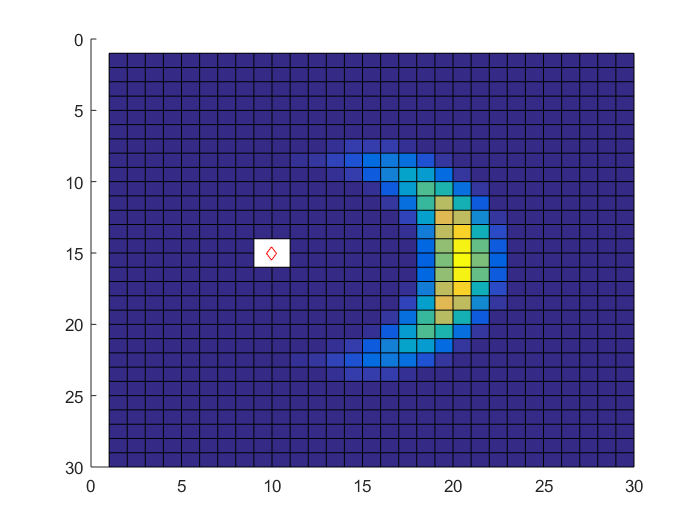
\includegraphics[width=0.95\linewidth]{figures/MotionModel_1}
		\caption{Odometry distribution for a $u_t$=[10 0] and an $a$=[0.01 0.01 0.01 0.1 0.001 0.001]}
	\end{minipage}%
	\hfill
	\begin{minipage}{.48\textwidth}
		\renewcommand\figurename{Fig.}
		\centering
		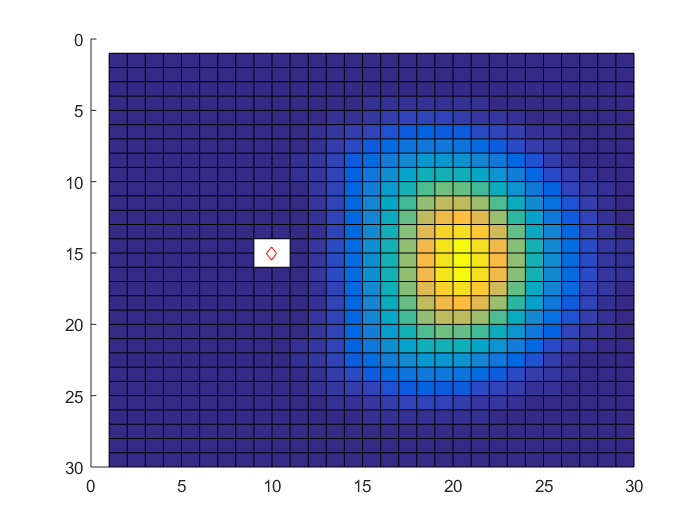
\includegraphics[width=0.95\linewidth]{figures/MotionModel_2}
		\caption{Odometry distribution for a $u_t$=[10 0] and an $a$=[0.1 0.1 0.01 0.01 0.001 0.001]}
	\end{minipage}%	
\end{figure}

It is suggested that you evaluate how big your movement commands $u_t$ are for every time step (they are dependant on the number of points \textit{path} has) adn the \textit{maximum velocity} set in the \textit{mstraj} function. Once you have an estimate, use the \textit{Motion\_Model\_Velocity\_Test} to see how your odometry distribution would look like for different motion error parameters $\alpha$. Try to fine-tune these values so that the simulated odometry error resembles the reality.

